\chapter{Referencial Teórico}
\label{ref}
\section{Software Analytics}
\label{ref:sof}
Durante muito tempo a disponibilidade de dados em projetos de software para análise foi um problema. Hoje em dia, com o auxílio da internet, dos projetos de software livre e das características pervasivas e ubíquas da computação, o volume de dados a serem analisados se tornou um problema. Processar e analisar esses dados manualmente se tornou inviável\cite{artAndScience}. \textcolor{red}{Atualizar esses números. Basta verificar no site do mozilla, github... } Atualmente, por exemplo, pesquisas mostraram que o \textit{Mozilla Firefox} teve 800.000 relatos de defeitos e outras plataformas como \textit{Sourcefoge.net} e o \textit{Github} hospedam 324.000 e 11.2 milhões de projetos, respectivamente\cite{informationNeeds}.

Para ser capaz de manipular essa grande quantidade de dados, muitos pesquisadores se voltaram para o uso e \textit{analytics}, ou seja, o uso de análises, dados e raciocínio sistemático para tomar decisões. Podemos definir \textit{Software Analytics} como: "A análise de dados de software para gerentes e engenheiros de software, com o objetivo de capacitar indivíduos e times de desenvolvimento, a ganhar e difundir conhecimento a partir de seus dados para tomar melhores decisões"\cite{informationNeeds}.

\todo[inline, backgroundcolor=yellow!20!white, bordercolor=red]{Reescrever o parágrafo acima. 1) A definição de software analytics não é um concenso; 2) software analytics foi uma evolução das pesquisas em mineração e análise em repositórios de software; 3) Software Analytics não existe para processar grandes volumes de dados (isso é propósito de Big Data) }

Hoje é comum empresas como Google, Facebook e Microsoft aplicarem métodos de análise de dados diariamente em seus projetos e produtos. Além disso, o número de conferências interessadas nos assuntos de mineração e análise de artefatos de software cresceu, destacando-se duas, a\textit{Mining Software Repositories} (MSR) e a \textit{PROMISE Conference on Repeatable Experimentes in Software Engineering}. Cada uma possui um foco diferente, sendo a MSR preocupada com a coleta dos dados, enquanto que a PROMISE com a eficácia e repetibilidade da análise de dados.

\todo[inline, backgroundcolor=yellow!20!white, bordercolor=red]{Melhorar a definição de software analytics. Não foram mencionados os trabalhos precurssores, os trabalhos atuais, os tipos de aplicação, tampouco o uso de algoritmos para busca e recuperação de informação em repositórios de software. }

\todo[inline, backgroundcolor=yellow!20!white, bordercolor=red]{Acrescentar aqui diferentes refências de trabalhos sobre mineração. Naquele livro do Zimmermman tem muitos trabalhos. Naquela revisão sitematica sobre software analytics tb. Ela nem foi citada nesse capitulo de referencial teorico...A caracterização de Software Analytics deixou a desejar.  }


\textcolor{red}{Por exemplo: Nos trabalhos.YYY foram utilizadas XXX técnicas, onde foi observado ZZZ}


A análise de dados obtidos de ferramentas de versionamento de código, como o Git, Bazaar, Subversion ou CVS pode trazer informações importantes a respeito da evolução de um projeto de software, por exemplo: o nível de engajamento dos desenvolvedores; o número de defeitos; a qualidade interna do produto; resultados de execução de testes, entre outros\cite{artAndScience}. O Github, uma das ferramentas mais utilizadas de versionamento de código-fonte atualmente, fornece uma api que permite a extração de dois tipos de dados: \todo{Perceba que há uma quebra no encadeamento das idéias. Da caracterizacao de software analytics, de repente aparece a api do github. Isso poderia ser uma subseção.}


\begin{itemize}
\item \textbf{Metadados:} Os metadados fornecidos são informações associadas a cada commit ou issue, são: criador(a), data, mensagem do commit ou issue, a branch, o repositório, e o escopo do commit ou issue. Além disso, na mensagem do commit podem haver referencias a outros
desenvolvedores, defeitos ou outros commits e issues.
\item \textbf{Snapshots:} O código fonte do projeto, que pode ser obtido em diferentes fases do desenvolvimento, já que a ferramente permite que um usuário avance ou retroceda dentro dos commits. Desta forma, é possível analisar o código de um projeto referente em vários períodos diferentes.
\end{itemize}

Abaixo, na figura~\ref{fig:github_api}, podemos ver o digrama de classes da API fornecida pelo
Github, com base nesta imagem, é possível ver que as issues e informações dos commiters
são exportadas a partir de um ponto comum de acesso.

\textcolor{red}{Retirar}

\begin{figure}[h]
    \centering
        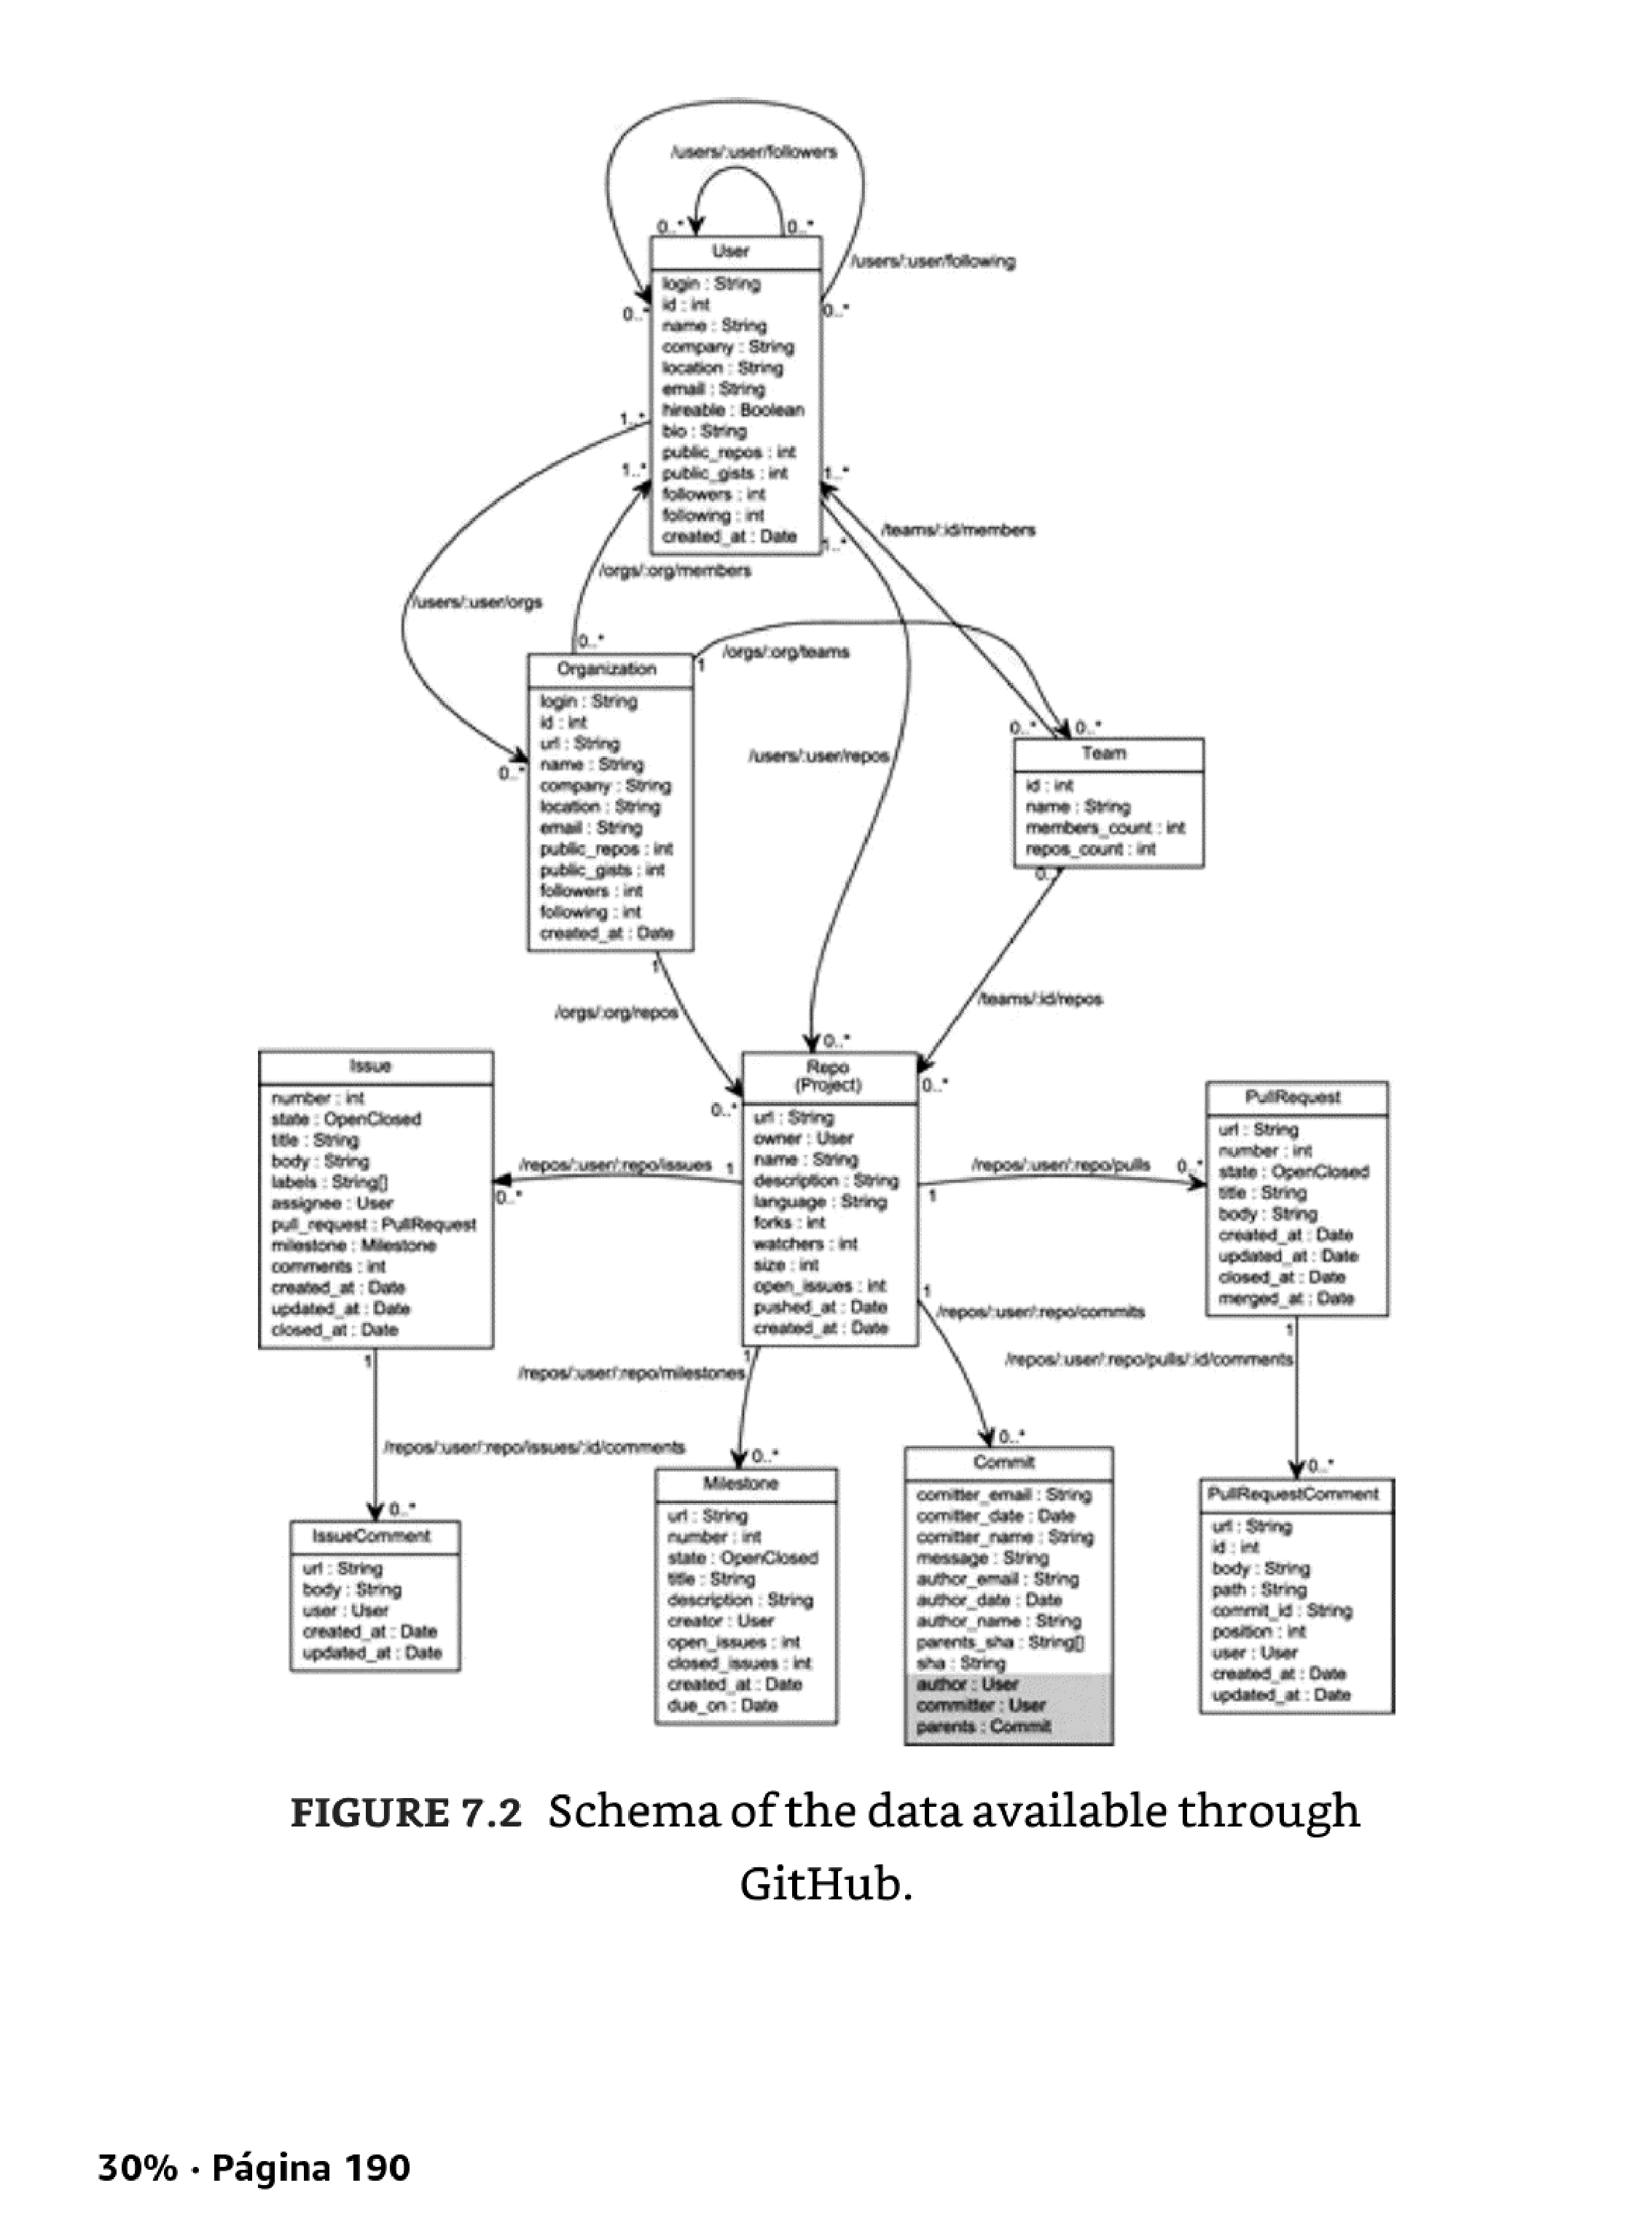
\includegraphics[keepaspectratio=true,scale=0.4]{figuras/github_api_diagram.eps}
    \caption{Representação UML da API do Github, extraído de \textcolor{red}{XXXXX ... Citar a fonte}}
    \label{fig:github_api}
\end{figure}

\todo[inline, backgroundcolor=yellow!20!white, bordercolor=red]{Retirar da figura 1 o caption em inglês. Essa figura na verdade está ilegível. Eu aumentei a escala para 50\% e ela passou a ocupar a página toda, além de continuar ilegível. Refaça a figura ou procure outra que seja legível}


Utilizando-se das informações mostradas na figura \ref{fig:github_api} é possível utilizar \textit{Software Analytics} para possibilitar uma melhor tomada de decisão em um repositório que utilize da ferramenta Github para organizar o trabalho. \textcolor{red}{Hein? Baseado em que você afirma que é possível tomar melhores decisões? Reescreva este parágrafo no sentido de que é possível recuperar dados a partir do repositório e que a partir disso análises podem ser realizadas para possivelmente apoiar a tomada de decisões}

\section{Centralidade de Redes}
\label{ref:cen}
Centralidade é um dos tópicos mais estudados na análise de redes sociais. Ela determina o grau de importância de um vértice dentre todos os outros dentro de uma rede. Na figura \ref{fig:centrality} é ilustrado um exemplo de centralidade. 
O conceito de centralidade de redes já foi aplicado a diversos contextos, dentre eles: investigar a influencia de redes inter organizacionais, estudos de relevância, vantagens em redes de troca, competência em organizações formais, oportunidades de emprego e diversos outros campos 
do mercado e ciência\cite{centrality}.

\todo[inline, backgroundcolor=yellow!20!white, bordercolor=red]{Agora deu nó mesmo!!! Novamente o encadeamento de idéias. Repare que em momento algum foi falado ou mesmo contextualizado sobre redes sociais e também sobre centralidade...}

\begin{figure}[h]
    \centering
        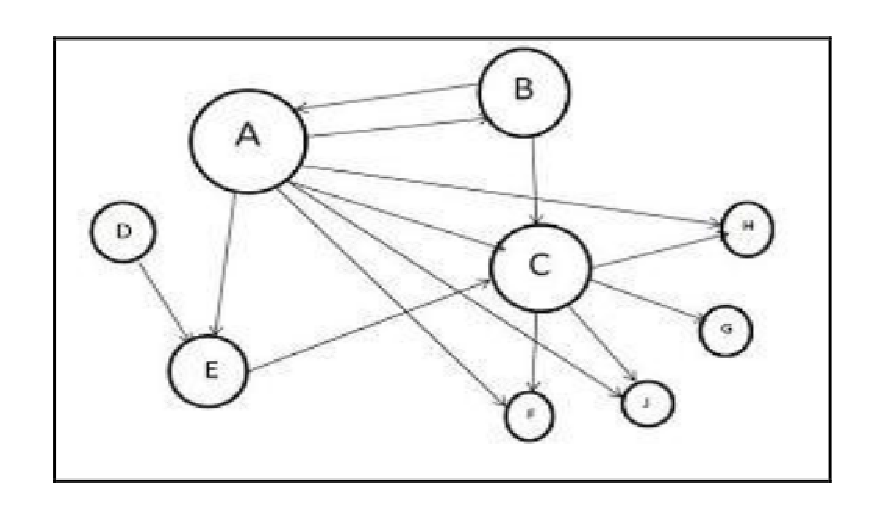
\includegraphics[keepaspectratio=true,scale=0.5]{figuras/centrality.eps}
    \caption{Exemplo de Relevância de um Nó em uma Rede}
    \label{fig:centrality}
\end{figure}

Diversos processos \textcolor{red}{Que tipo de processos?} comumente encontrados no dia-a-dia são caracterizados por um fluxo. Esses processos diferem em dimensão e tipo, mas ainda assim podem ser comparados e exemplificados. Considerando que os processos de XXXX representam um fluxo, então podemos descrevê-los sob a perspectiva da Teoria dos Grafos\cite{ceflow}. Por exemplo:

\begin{itemize}
\item Dinheiro: Considere uma moeda, ou nota de um dólar, que se move pela
economia e muda de mãos a cada transação. Uma nota é indivisível e só pode estar em um lugar em um determinado período de tempo. Na perspectiva da teoria dos grafos, a movimentação de uma nota em uma rede pode ser feita como um \textit{passeio (Walk)}, sendo, desta forma, representado como um processo de Markov. \textcolor{red}{Referência}
\item Fofoca: Imagine uma informação privada que passa por uma rede
de empregados de uma empresa. Diferentemente de uma moeda, essa mesma informação pode estar em diversos locais diferentes em um determinado período de tempo, se replicando a cada pessoa que passa a ter acesso a informação, mas geralmente não atravessa o mesmo vértice mais de uma vez, apesar de poder visitar o mesmo nó mais de uma vez. A movimentação desta informação em grafo pode ser representada como uma trilha. \textcolor{red}{Referência}
\item E-mail: Um vírus, o spam de e-mail, que envia mensagens a todos os
contatos de uma pessoa simultaneamente pode ser considerado um processo de fluxo. \textcolor{red}{Ficou meio confuso, principalmente no início da oração}. Um e-mail pode ser representado como uma trilha da mesma forma que é realizado com uma informação, já que compartilha propriedades semelhantes, como existir em diversos locais ao mesmo tempo, e geralmente, os e-mails não passam pelo mesmo vértice, ou caminho, duas vezes.
\item Infecções: O caso de uma infecção em que o hospedeiro ficou imune.
A infecção vão passar por duplicação de pessoa a pessoa, mas nunca vai voltar a infectar aqueles que já se tornaram imunes.
\item Pacotes: Um pacote de rede tem a característica de possuir
um remetente e um destinatário. Normalmente é preferível que o pacote percorra o menor caminho possível até chegar ao seu destino. Dessa forma, a movimentação do pacote deve seguir o caminho geodésico pela rede \textcolor{red}{Colocar uma nota de rodapé com a definição de caminho geodésico} e roteadores. 
\end{itemize}

\todo[inline, backgroundcolor=yellow!20!white, bordercolor=red]{Aqui faltou um parágrafo para alinhar a idéia desses exemplos com o foco que você pretende dar no seu caso em particular da investigação sobre centralidade.}

Ao longo dos anos, diferentes métodos de medida de centralidade foram criados, entre eles: \textcolor{red}{Citar as referências}
Centralidade de Grau, Proximidade \textit{(Closeness)}, Intermediação \textit{(Betweenness)}, Autovetor \textit{(Eigen Vector)}, Informação, Intermediação de Fluxo, \textit{Rush Index}, Medidas de Influencia de Katz, Hubbell, Hoede e Taylor. Estes métodos diferem nas suposições
iniciais que fazem para alcançar o objetivo de determinar o nó com maior importância, por exemplo, o algoritmo de Freeman de proximidade e intermediação conta apenas os caminhos geodésicos entre os nós, assumindo que qualquer fluxo que percorra uma rede, siga sempre pelo caminho mais curto.Outros algoritmos como a centralidade de autovetor de Bonacich conta travessias, o que assume que as trajetórias podem ser sinuosas, atravessando nós e arestas repetidas vezes até chegar ao destino\cite{centrality}.

\todo[inline, backgroundcolor=yellow!20!white, bordercolor=red]{Ok, mas qual a relação de centralidade com software analytics? e também o ranqueamento de páginas? Você não acredita que seria melhor essa discussão de centralidade na seção do Ranqueamento de Páginas?}

\section{Ranqueamento de Páginas}
\label{ref:ran}
O algoritmo de ranqueamento de páginas foi criado por Larry Page e Sergey em 1996. Ele permite calcular a importância relativa de páginas da web e tem aplicações em mecanismos de busca, estimativas de trafego e navegação na web. O algoritmo foi criado com o intuito de prover uma solução de busca de informações na web a partir da estrutura dos links, usada no hipertexto da web. \cite{pageRank}.

A premissa do algoritmo de ranqueamento de páginas é que cada página na web possui um número de links de saída e de entrada, e que páginas com um grande número de links são mais importantes do que as com poucos links. Além disso, o algoritmo também leva em consideração a relevância dos links de entrada de uma página, ou seja, se uma página da web possui um link de entrada que possui uma alta relevância, essa página tende a ser mais importante que outra que possua vários links mas que vieram de lugares mais obscuros \textcolor{red}{o que é mais obscuros?}.

A função de ranqueamento de páginas é definida na seguinte forma:

Seja $x$ uma página da web. Então
\begin{itemize}
    \item $L(x)$ é o conjunto de websites que possuem link para $x$
    \item $C(y)$ é o grau de entrada de $y$
    \item $\alpha$ é a probabilidade de um pulo aleatório
    \item $N$ é o número total de websites
\end{itemize}
\[\displaystyle PR(x) := \alpha \left ( \frac{1}{N} \right ) + (1-\alpha) \sum_{y\in L(x)} \frac{PR(y)}{C(y)}\]

Aplicando a equação acima, é possível obter o ranque de uma página, dado um conjunto de web-sites avaliados. \textcolor{red}{Explique melhor a função/aplicação.}

 Na figura \ref{fig:page_rank} é apresentado um exemplo como a relevância de uma página influencia as páginas seguintes.

\begin{figure}[h]
    \centering
        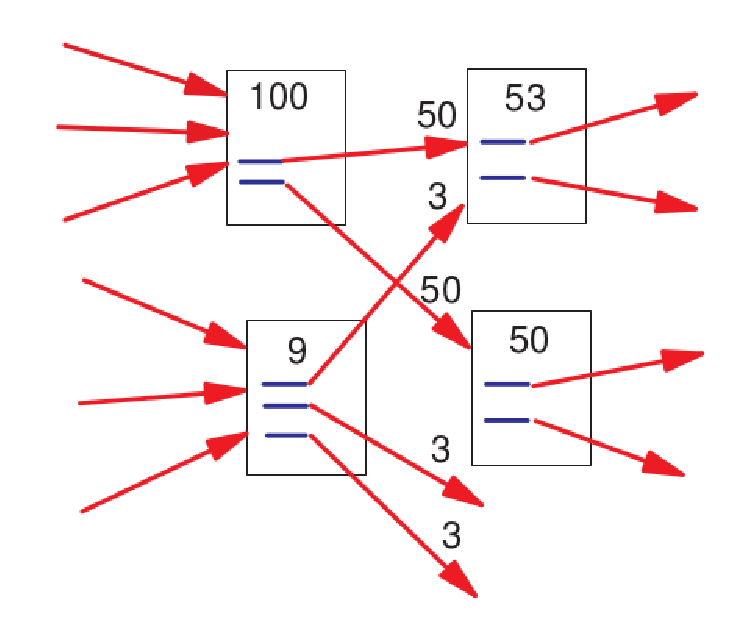
\includegraphics[keepaspectratio=true,scale=0.5]{figuras/page_rank.eps}
    \caption{Simplificação do Cálculo de Ranqueamento de Páginas}
    \label{fig:page_rank}
\end{figure}

\begin{figure}[h]
    \centering
        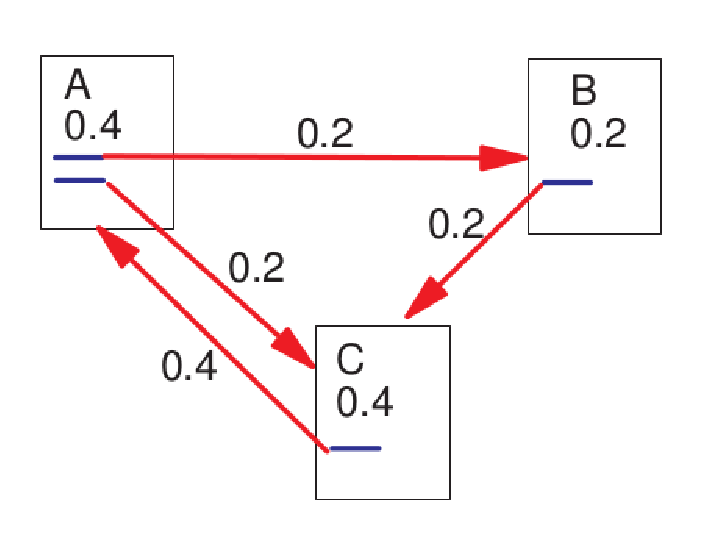
\includegraphics[keepaspectratio=true,scale=0.5]{figuras/page_rank2.eps}
    \caption{Simplificação do Cálculo de Ranqueamento de Páginas}
    \label{fig:page_rank2}
\end{figure}

Na figura \ref{fig:page_rank} é ilustrado como o ranqueamento de páginas se divide através das paginas e como ele contribui para o ranque das páginas seguintes. Já na figura \ref{fig:page_rank2} é ilustrado como um estado estável pode ser alcançado depois que o algoritmo é executado em um conjunto de páginas. 

\todo[inline, backgroundcolor=yellow!20!white, bordercolor=red]{As figuras estão sendo todas deslocadas para o final do cap. Fixe a posição delas no texto}

\todo[inline, backgroundcolor=yellow!20!white, bordercolor=red]{Conforme eu já havia apontado na apresentação, eu esperava que o texto melhor explicasse as figuras. Elas (as figuras) não são autoexplicativas. Então explique tanto a figura 3, 4 e 5}


\begin{figure}[h]
    \centering
        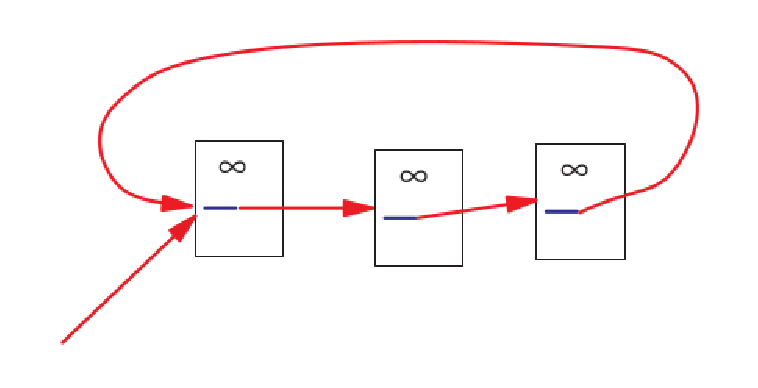
\includegraphics[keepaspectratio=true,scale=0.5]{figuras/page_rank3.eps}
    \caption{Loop de Ranqueamento}
    \label{fig:page_rank3}
\end{figure}

Um dos problemas dessa função de ranqueamento, é que caso duas páginas da web que apontem uma para outra, e uma terceira aponte para qualquer uma destas, o loop vai acumular ranque porém, nunca vai distribuir isso para nenhuma outra página seguinte. Na ilustração apresentada na figura \ref{fig:page_rank3}, possível observar esse fenômeno.

\todo[inline, backgroundcolor=yellow!20!white, bordercolor=red]{Incluir um parágrafo que faça o link de idéias entre esse capítulo e o próximo.}

\textit{Faltou sessão para falar sobre planejamento de release e como organizar issues na wiki}
\textit{Capitulo 19 do livro}
